\documentclass[11pt,a4paper]{article}

% Define page geometry
\usepackage{geometry}
\geometry{left=2.2cm,
	right=2.2cm,
	top=2.2cm,
	bottom=2cm}
\parskip 0.15cm
\setlength{\parindent}{0cm}
\usepackage{pdflscape}
\usepackage[document]{ragged2e}

% Set font
\usepackage[T1]{fontenc}

\usepackage{framed}

% Image handling
\usepackage{graphics} % Insert images easily
\usepackage{graphicx} % Extended image support

\makeatletter
	\g@addto@macro\@floatboxreset\centering % Automatically centre images (floats)
\makeatother

\graphicspath{ {img/} }
\usepackage{float} % Graphics placement [H] [H!] arguments
\usepackage{subfig} % Compound figures

% Tables
\usepackage{multirow}
\usepackage{longtable}

% Bibliography management
\usepackage[UKenglish]{babel}
\usepackage[natbibapa]{apacite}
\bibliographystyle{apacite}

% Text formatting
\usepackage{url} % Allow nice formatting of URLs in text

\usepackage{enumerate} % Enumerated lists

\usepackage{lineno} % Line numbers

\usepackage{textcomp}
\newcommand{\textapprox}{\raisebox{0.5ex}{\texttildelow}} % Command for a good tilde

\usepackage{siunitx}
\usepackage{amsmath}

\usepackage{xcolor}
\newcommand{\TODO}[1]{\textcolor{red}{\textbf{#1}}}  % \TODO{NOTE TO SELF WRITTEN IN RED}

\input{code_format}

\usepackage[breaklinks]{hyperref}
\definecolor{links}{RGB}{0,0,0}
\hypersetup{
	breaklinks,
	colorlinks=true,
	linkcolor=links,
	anchorcolor=links,
	citecolor=links,
	filecolor=links,
	menucolor=links,
	runcolor=links,
	urlcolor=links,
	pdfauthor={John L. Godlee}
}
\def\subsectionautorefname{section}
\def\subsubsectionautorefname{section}
% \usepackage{biblatex}

\usepackage{dcolumn}
\usepackage{multirow}
\usepackage{tikz}
\usetikzlibrary{calc,arrows,positioning,shapes,shapes.gates.logic.US,trees}
\usepackage{pdflscape}
\usepackage{longtable}
\usepackage{fmtcount}

\linenumbers
\linespread{1.25}

\newcommand{\titletext}{Structural diversity and tree density drives variation in the biodiversity-ecosystem function relationship of woodlands and savannas}

\begin{document}

{\Large{Title: \titletext{}}}

\section{Appendix 1 - Frequency distribution of observed variables} \label{appendixa}

\begin{figure}[H]
\centering
	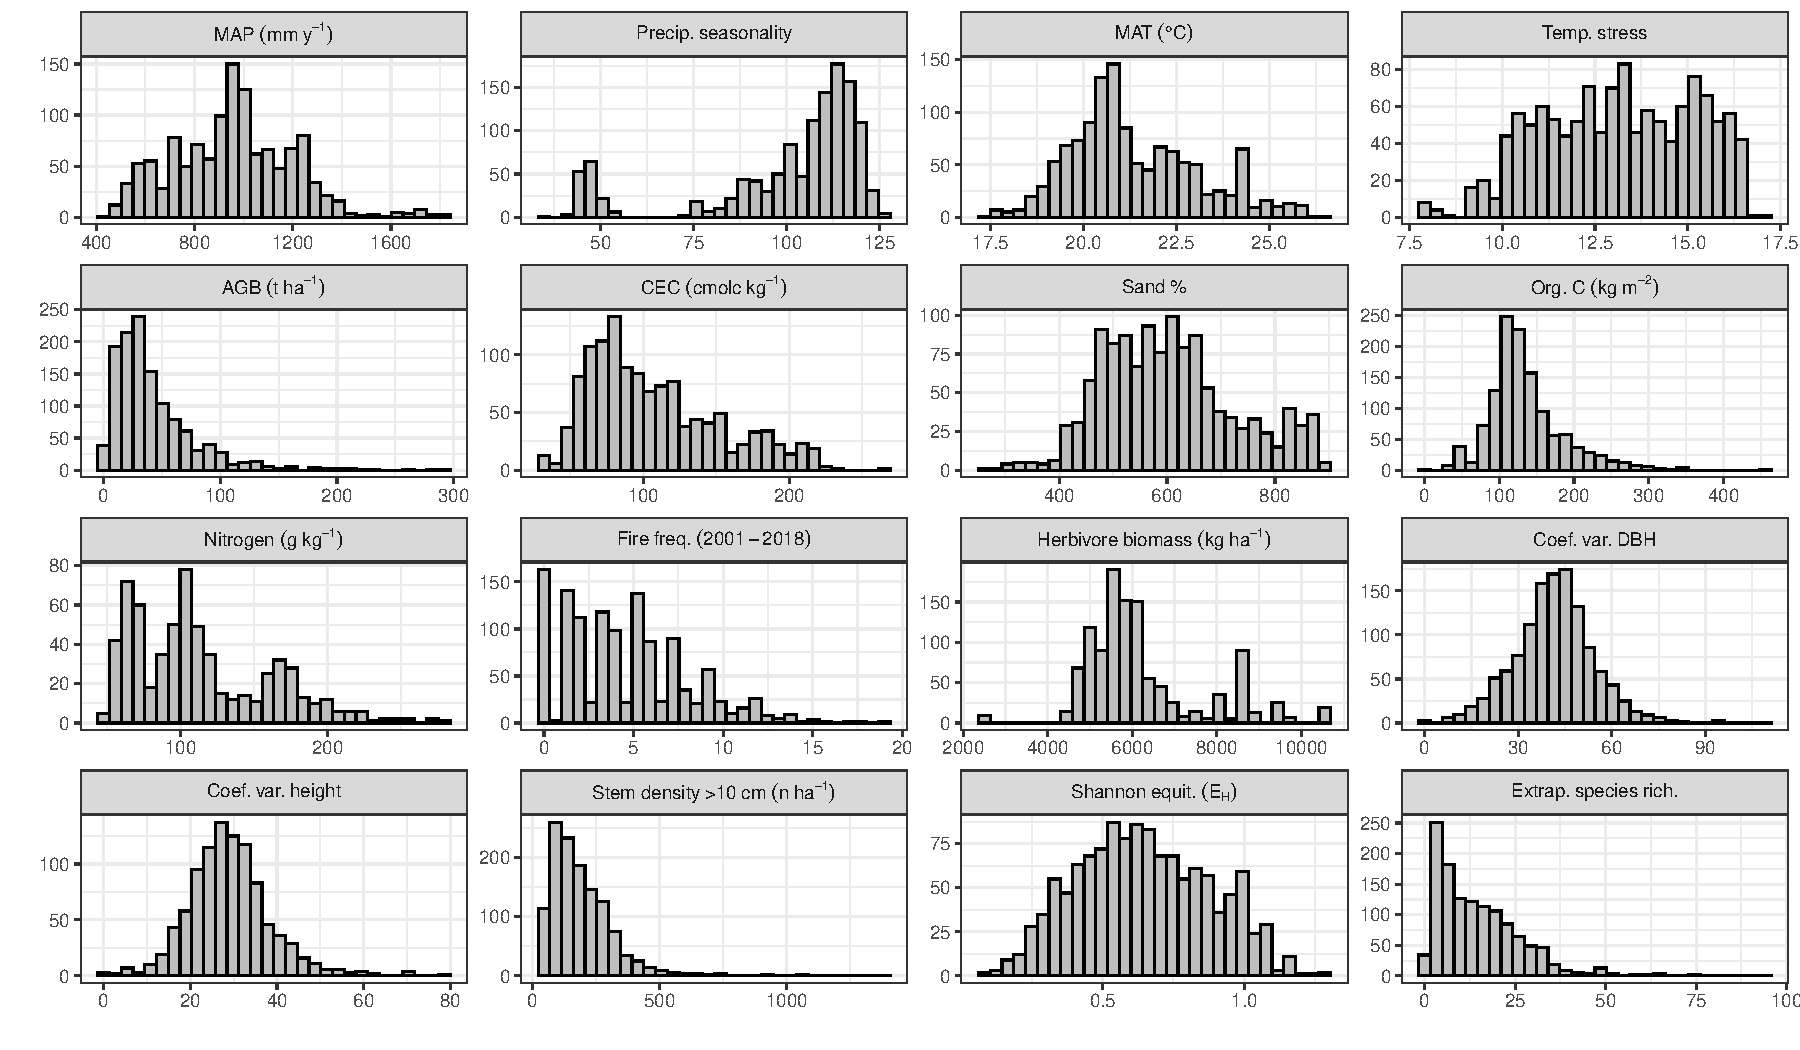
\includegraphics[width=\textwidth]{hist_raw}
	\caption{Histograms of raw untransformed observed variables used in final analyses.}
	\label{hist_raw}
\end{figure}

\begin{figure}[H]
\centering
	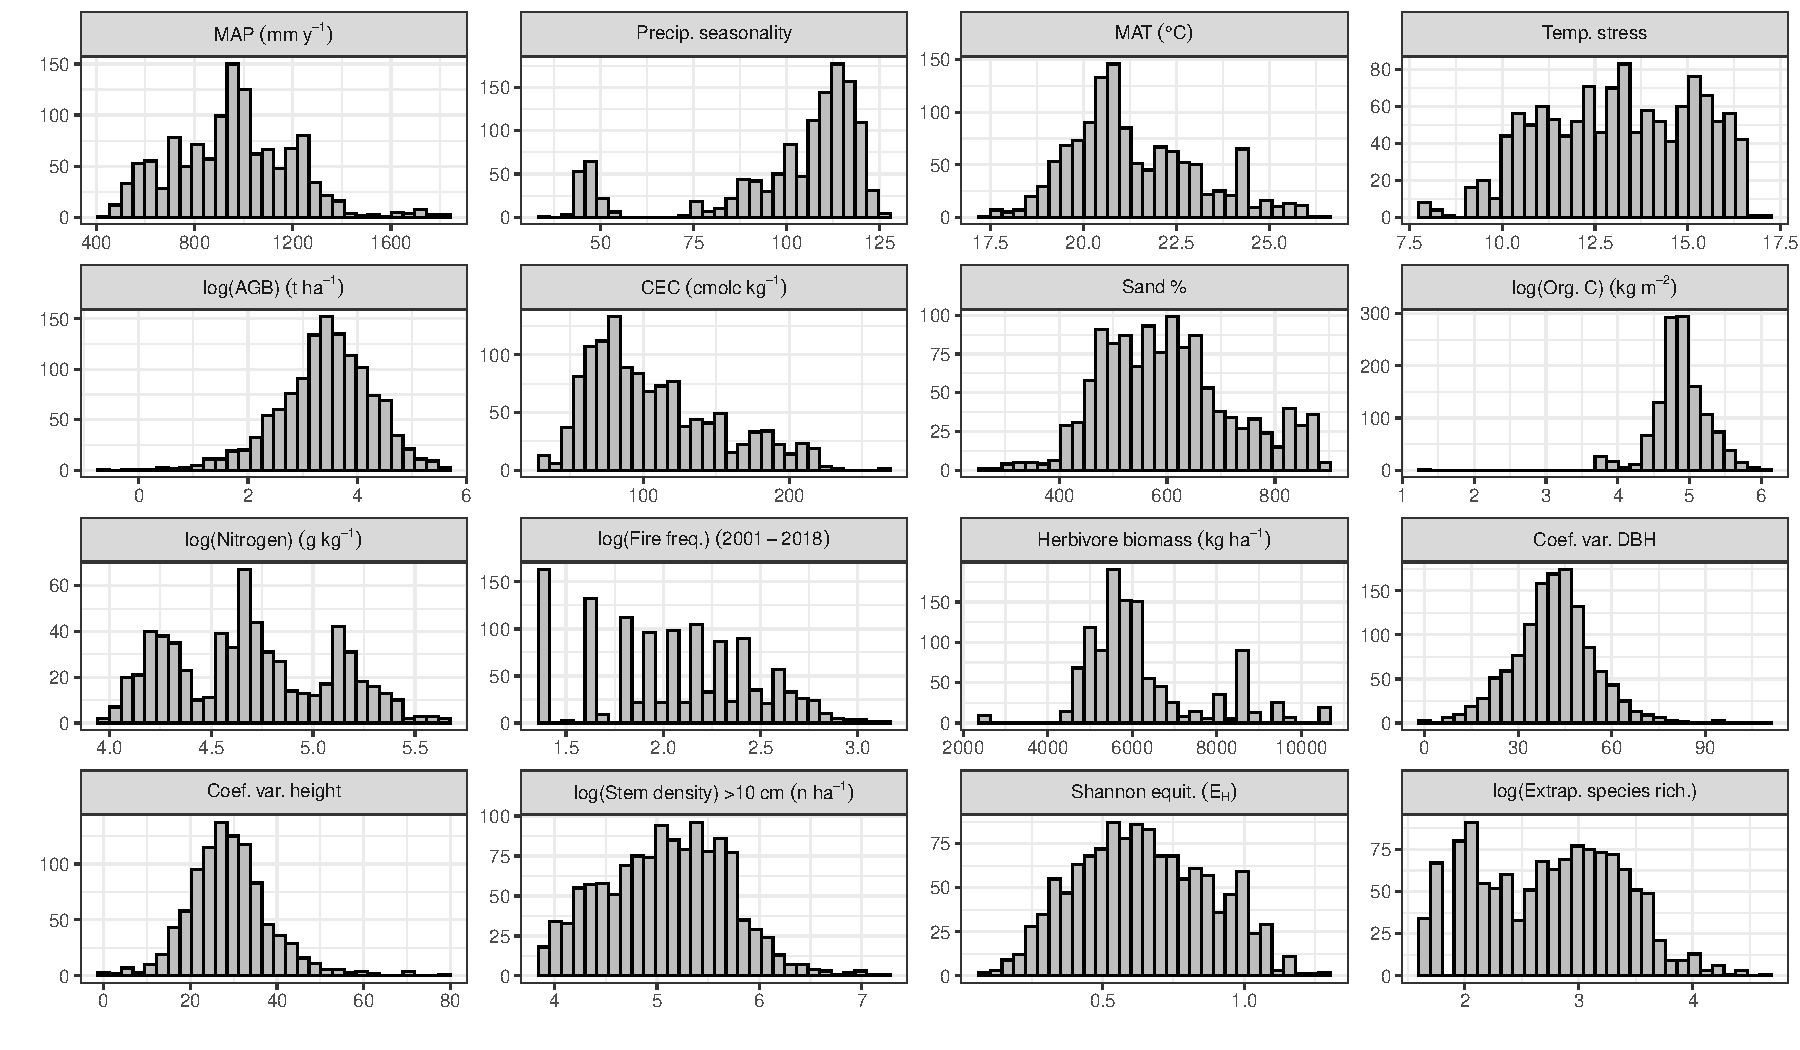
\includegraphics[width=\textwidth]{hist_trans}
	\caption{Histograms of observed variables transformed to achieve a normal frequency distribution.}
	\label{hist_trans}
\end{figure}

\appendix{}
\section{Appendix 2 - Table of correlation fit statistics} \label{appendixb}


% Table created by stargazer v.5.2.2 by Marek Hlavac, Harvard University. E-mail: hlavac at fas.harvard.edu
% Date and time: Sat, Jan 30, 2021 - 13:12:29
\begin{longtable}{ccccccc}
  	\caption{Table of correlation fit statistics for all observed variables used in final analyses, showing the Pearson correlation coefficient ($r$), the correlation confidence interval upper and lower bounds, number of plots used in the correlation (n), and the p-value of the correlation.} 
\\[-1.8ex]\hline 
\hline \\[-1.8ex] 
X & Y & $r$ & Lower bound & Upper bound & n & Prob. \\ 
\hline \\[-1.8ex] 
\endhead
Soil CEC & Soil C & $0.260$ & $0.210$ & $0.310$ & $1239$ & p \textless 0.01 \\ 
Soil N & Soil C & $0.850$ & $0.820$ & $0.870$ & $644$ & p \textless 0.01 \\ 
Fire freq. & Soil C & $$-$0.070$ & $$-$0.130$ & $$-$0.010$ & $1239$ & p \textless 0.05 \\ 
MAP & Soil C & $0.510$ & $0.460$ & $0.550$ & $1239$ & p \textless 0.01 \\ 
Precip. seas. & Soil C & $$-$0.560$ & $$-$0.600$ & $$-$0.520$ & $1239$ & p \textless 0.01 \\ 
Temp. stress & Soil C & $$-$0.630$ & $$-$0.670$ & $$-$0.600$ & $1239$ & p \textless 0.01 \\ 
Sand \% & Soil C & $$-$0.570$ & $$-$0.610$ & $$-$0.540$ & $1239$ & p \textless 0.01 \\ 
Extrap. sp. rich. & Soil C & $0.250$ & $0.200$ & $0.300$ & $1239$ & p \textless 0.01 \\ 
Shannon equit & Soil C & $0.230$ & $0.180$ & $0.280$ & $1239$ & p \textless 0.01 \\ 
Tree height CV & Soil C & $0.230$ & $0.170$ & $0.290$ & $981$ & p \textless 0.01 \\ 
DBH CV & Soil C & $0.160$ & $0.110$ & $0.220$ & $1237$ & p \textless 0.01 \\ 
Stem density & Soil C & $0.070$ & $0.020$ & $0.130$ & $1239$ & p \textless 0.05 \\ 
AGB & Soil C & $0.260$ & $0.210$ & $0.320$ & $1239$ & p \textless 0.01 \\ 
Soil N & Soil CEC & $0.440$ & $0.370$ & $0.500$ & $644$ & p \textless 0.01 \\ 
Fire freq. & Soil CEC & $$-$0.470$ & $$-$0.510$ & $$-$0.430$ & $1239$ & p \textless 0.01 \\ 
MAP & Soil CEC & $$-$0.280$ & $$-$0.330$ & $$-$0.220$ & $1239$ & p \textless 0.01 \\ 
Precip. seas. & Soil CEC & $$-$0.710$ & $$-$0.730$ & $$-$0.680$ & $1239$ & p \textless 0.01 \\ 
Temp. stress & Soil CEC & $$-$0.250$ & $$-$0.300$ & $$-$0.200$ & $1239$ & p \textless 0.01 \\ 
Sand \% & Soil CEC & $$-$0.210$ & $$-$0.270$ & $$-$0.160$ & $1239$ & p \textless 0.01 \\ 
Extrap. sp. rich. & Soil CEC & $$-$0.380$ & $$-$0.430$ & $$-$0.330$ & $1239$ & p \textless 0.01 \\ 
Shannon equit & Soil CEC & $$-$0.090$ & $$-$0.150$ & $$-$0.040$ & $1239$ & p \textless 0.01 \\ 
Tree height CV & Soil CEC & $$-$0.110$ & $$-$0.170$ & $$-$0.050$ & $981$ & p \textless 0.01 \\ 
DBH CV & Soil CEC & $$-$0.010$ & $$-$0.070$ & $0.040$ & $1237$ & p = 0.62 \\ 
Stem density & Soil CEC & $$-$0.020$ & $$-$0.080$ & $0.030$ & $1239$ & p = 0.43 \\ 
AGB & Soil CEC & $$-$0.040$ & $$-$0.090$ & $0.020$ & $1239$ & p = 0.17 \\ 
Fire freq. & Soil N & $$-$0.250$ & $$-$0.320$ & $$-$0.180$ & $644$ & p \textless 0.01 \\ 
MAP & Soil N & $0.370$ & $0.300$ & $0.440$ & $644$ & p \textless 0.01 \\ 
Precip. seas. & Soil N & $$-$0.760$ & $$-$0.790$ & $$-$0.730$ & $644$ & p \textless 0.01 \\ 
Temp. stress & Soil N & $$-$0.800$ & $$-$0.820$ & $$-$0.770$ & $644$ & p \textless 0.01 \\ 
Sand \% & Soil N & $$-$0.660$ & $$-$0.700$ & $$-$0.610$ & $644$ & p \textless 0.01 \\ 
Extrap. sp. rich. & Soil N & $0.440$ & $0.380$ & $0.500$ & $644$ & p \textless 0.01 \\ 
Shannon equit & Soil N & $0.350$ & $0.280$ & $0.420$ & $644$ & p \textless 0.01 \\ 
Tree height CV & Soil N & $0.270$ & $0.180$ & $0.360$ & $386$ & p \textless 0.01 \\ 
DBH CV & Soil N & $0.260$ & $0.180$ & $0.330$ & $642$ & p \textless 0.01 \\ 
Stem density & Soil N & $$-$0.030$ & $$-$0.110$ & $0.050$ & $644$ & p = 0.47 \\ 
AGB & Soil N & $0.310$ & $0.240$ & $0.380$ & $644$ & p \textless 0.01 \\ 
MAP & Fire freq. & $0.370$ & $0.320$ & $0.420$ & $1239$ & p \textless 0.01 \\ 
Precip. seas. & Fire freq. & $0.360$ & $0.310$ & $0.410$ & $1239$ & p \textless 0.01 \\ 
Temp. stress & Fire freq. & $0.210$ & $0.160$ & $0.260$ & $1239$ & p \textless 0.01 \\ 
Sand \% & Fire freq. & $0.060$ & $0$ & $0.110$ & $1239$ & p \textless 0.05 \\ 
Extrap. sp. rich. & Fire freq. & $0.380$ & $0.340$ & $0.430$ & $1239$ & p \textless 0.01 \\ 
Shannon equit & Fire freq. & $0.120$ & $0.070$ & $0.180$ & $1239$ & p \textless 0.01 \\ 
Tree height CV & Fire freq. & $0.150$ & $0.090$ & $0.220$ & $981$ & p \textless 0.01 \\ 
DBH CV & Fire freq. & $0.120$ & $0.070$ & $0.180$ & $1237$ & p \textless 0.01 \\ 
Stem density & Fire freq. & $$-$0.020$ & $$-$0.070$ & $0.040$ & $1239$ & p = 0.52 \\ 
AGB & Fire freq. & $0.030$ & $$-$0.030$ & $0.080$ & $1239$ & p = 0.33 \\ 
Precip. seas. & MAP & $$-$0.070$ & $$-$0.120$ & $$-$0.010$ & $1239$ & p \textless 0.05 \\ 
Temp. stress & MAP & $$-$0.490$ & $$-$0.530$ & $$-$0.440$ & $1239$ & p \textless 0.01 \\ 
Sand \% & MAP & $$-$0.330$ & $$-$0.380$ & $$-$0.280$ & $1239$ & p \textless 0.01 \\ 
Extrap. sp. rich. & MAP & $0.410$ & $0.360$ & $0.450$ & $1239$ & p \textless 0.01 \\ 
Shannon equit & MAP & $0.150$ & $0.100$ & $0.200$ & $1239$ & p \textless 0.01 \\ 
Tree height CV & MAP & $0.250$ & $0.190$ & $0.300$ & $981$ & p \textless 0.01 \\ 
DBH CV & MAP & $0.110$ & $0.060$ & $0.170$ & $1237$ & p \textless 0.01 \\ 
Stem density & MAP & $0.020$ & $$-$0.030$ & $0.080$ & $1239$ & p = 0.47 \\ 
AGB & MAP & $0.240$ & $0.180$ & $0.290$ & $1239$ & p \textless 0.01 \\ 
Temp. stress & Precip. seas. & $0.500$ & $0.450$ & $0.540$ & $1239$ & p \textless 0.01 \\ 
Sand \% & Precip. seas. & $0.310$ & $0.260$ & $0.360$ & $1239$ & p \textless 0.01 \\ 
Extrap. sp. rich. & Precip. seas. & $0.120$ & $0.070$ & $0.180$ & $1239$ & p \textless 0.01 \\ 
Shannon equit & Precip. seas. & $$-$0.070$ & $$-$0.120$ & $$-$0.010$ & $1239$ & p \textless 0.05 \\ 
Tree height CV & Precip. seas. & $$-$0.050$ & $$-$0.110$ & $0.010$ & $981$ & p = 0.11 \\ 
DBH CV & Precip. seas. & $$-$0.100$ & $$-$0.150$ & $$-$0.040$ & $1237$ & p \textless 0.01 \\ 
Stem density & Precip. seas. & $$-$0.040$ & $$-$0.100$ & $0.010$ & $1239$ & p = 0.12 \\ 
AGB & Precip. seas. & $$-$0.180$ & $$-$0.230$ & $$-$0.130$ & $1239$ & p \textless 0.01 \\ 
Sand \% & Temp. stress & $0.300$ & $0.250$ & $0.350$ & $1239$ & p \textless 0.01 \\ 
Extrap. sp. rich. & Temp. stress & $$-$0.130$ & $$-$0.180$ & $$-$0.070$ & $1239$ & p \textless 0.01 \\ 
Shannon equit & Temp. stress & $$-$0.130$ & $$-$0.180$ & $$-$0.070$ & $1239$ & p \textless 0.01 \\ 
Tree height CV & Temp. stress & $$-$0.140$ & $$-$0.200$ & $$-$0.080$ & $981$ & p \textless 0.01 \\ 
DBH CV & Temp. stress & $$-$0.040$ & $$-$0.100$ & $0.010$ & $1237$ & p = 0.12 \\ 
Stem density & Temp. stress & $0.030$ & $$-$0.020$ & $0.090$ & $1239$ & p = 0.27 \\ 
AGB & Temp. stress & $$-$0.170$ & $$-$0.220$ & $$-$0.110$ & $1239$ & p \textless 0.01 \\ 
Extrap. sp. rich. & Sand \% & $$-$0.270$ & $$-$0.320$ & $$-$0.220$ & $1239$ & p \textless 0.01 \\ 
Shannon equit & Sand \% & $$-$0.210$ & $$-$0.260$ & $$-$0.160$ & $1239$ & p \textless 0.01 \\ 
Tree height CV & Sand \% & $$-$0.240$ & $$-$0.300$ & $$-$0.180$ & $981$ & p \textless 0.01 \\ 
DBH CV & Sand \% & $$-$0.160$ & $$-$0.210$ & $$-$0.100$ & $1237$ & p \textless 0.01 \\ 
Stem density & Sand \% & $$-$0.140$ & $$-$0.190$ & $$-$0.080$ & $1239$ & p \textless 0.01 \\ 
AGB & Sand \% & $$-$0.220$ & $$-$0.270$ & $$-$0.160$ & $1239$ & p \textless 0.01 \\ 
Shannon equit & Extrap. sp. rich. & $0.600$ & $0.560$ & $0.630$ & $1249$ & p \textless 0.01 \\ 
Tree height CV & Extrap. sp. rich. & $0.310$ & $0.250$ & $0.360$ & $981$ & p \textless 0.01 \\ 
DBH CV & Extrap. sp. rich. & $0.320$ & $0.260$ & $0.360$ & $1247$ & p \textless 0.01 \\ 
Stem density & Extrap. sp. rich. & $0.230$ & $0.170$ & $0.280$ & $1249$ & p \textless 0.01 \\ 
AGB & Extrap. sp. rich. & $0.330$ & $0.280$ & $0.380$ & $1249$ & p \textless 0.01 \\ 
Tree height CV & Shannon equit & $0.140$ & $0.070$ & $0.200$ & $981$ & p \textless 0.01 \\ 
DBH CV & Shannon equit & $0.230$ & $0.170$ & $0.280$ & $1247$ & p \textless 0.01 \\ 
Stem density & Shannon equit & $0.410$ & $0.360$ & $0.450$ & $1249$ & p \textless 0.01 \\ 
AGB & Shannon equit & $0.380$ & $0.330$ & $0.420$ & $1249$ & p \textless 0.01 \\ 
DBH CV & Tree height CV & $0.490$ & $0.440$ & $0.540$ & $981$ & p \textless 0.01 \\ 
Stem density & Tree height CV & $0$ & $$-$0.060$ & $0.060$ & $981$ & p = 0.95 \\ 
AGB & Tree height CV & $0.240$ & $0.180$ & $0.300$ & $981$ & p \textless 0.01 \\ 
Stem density & DBH CV & $0.110$ & $0.050$ & $0.160$ & $1247$ & p \textless 0.01 \\ 
AGB & DBH CV & $0.440$ & $0.400$ & $0.490$ & $1247$ & p \textless 0.01 \\ 
AGB & Stem density & $0.570$ & $0.530$ & $0.610$ & $1249$ & p \textless 0.01 \\ 
\hline \\[-1.8ex] 
\end{longtable} 


\section{Appendix 3 - Bivariate relationships of model variables} \label{appendixc}

\begin{figure}[H]
\centering
	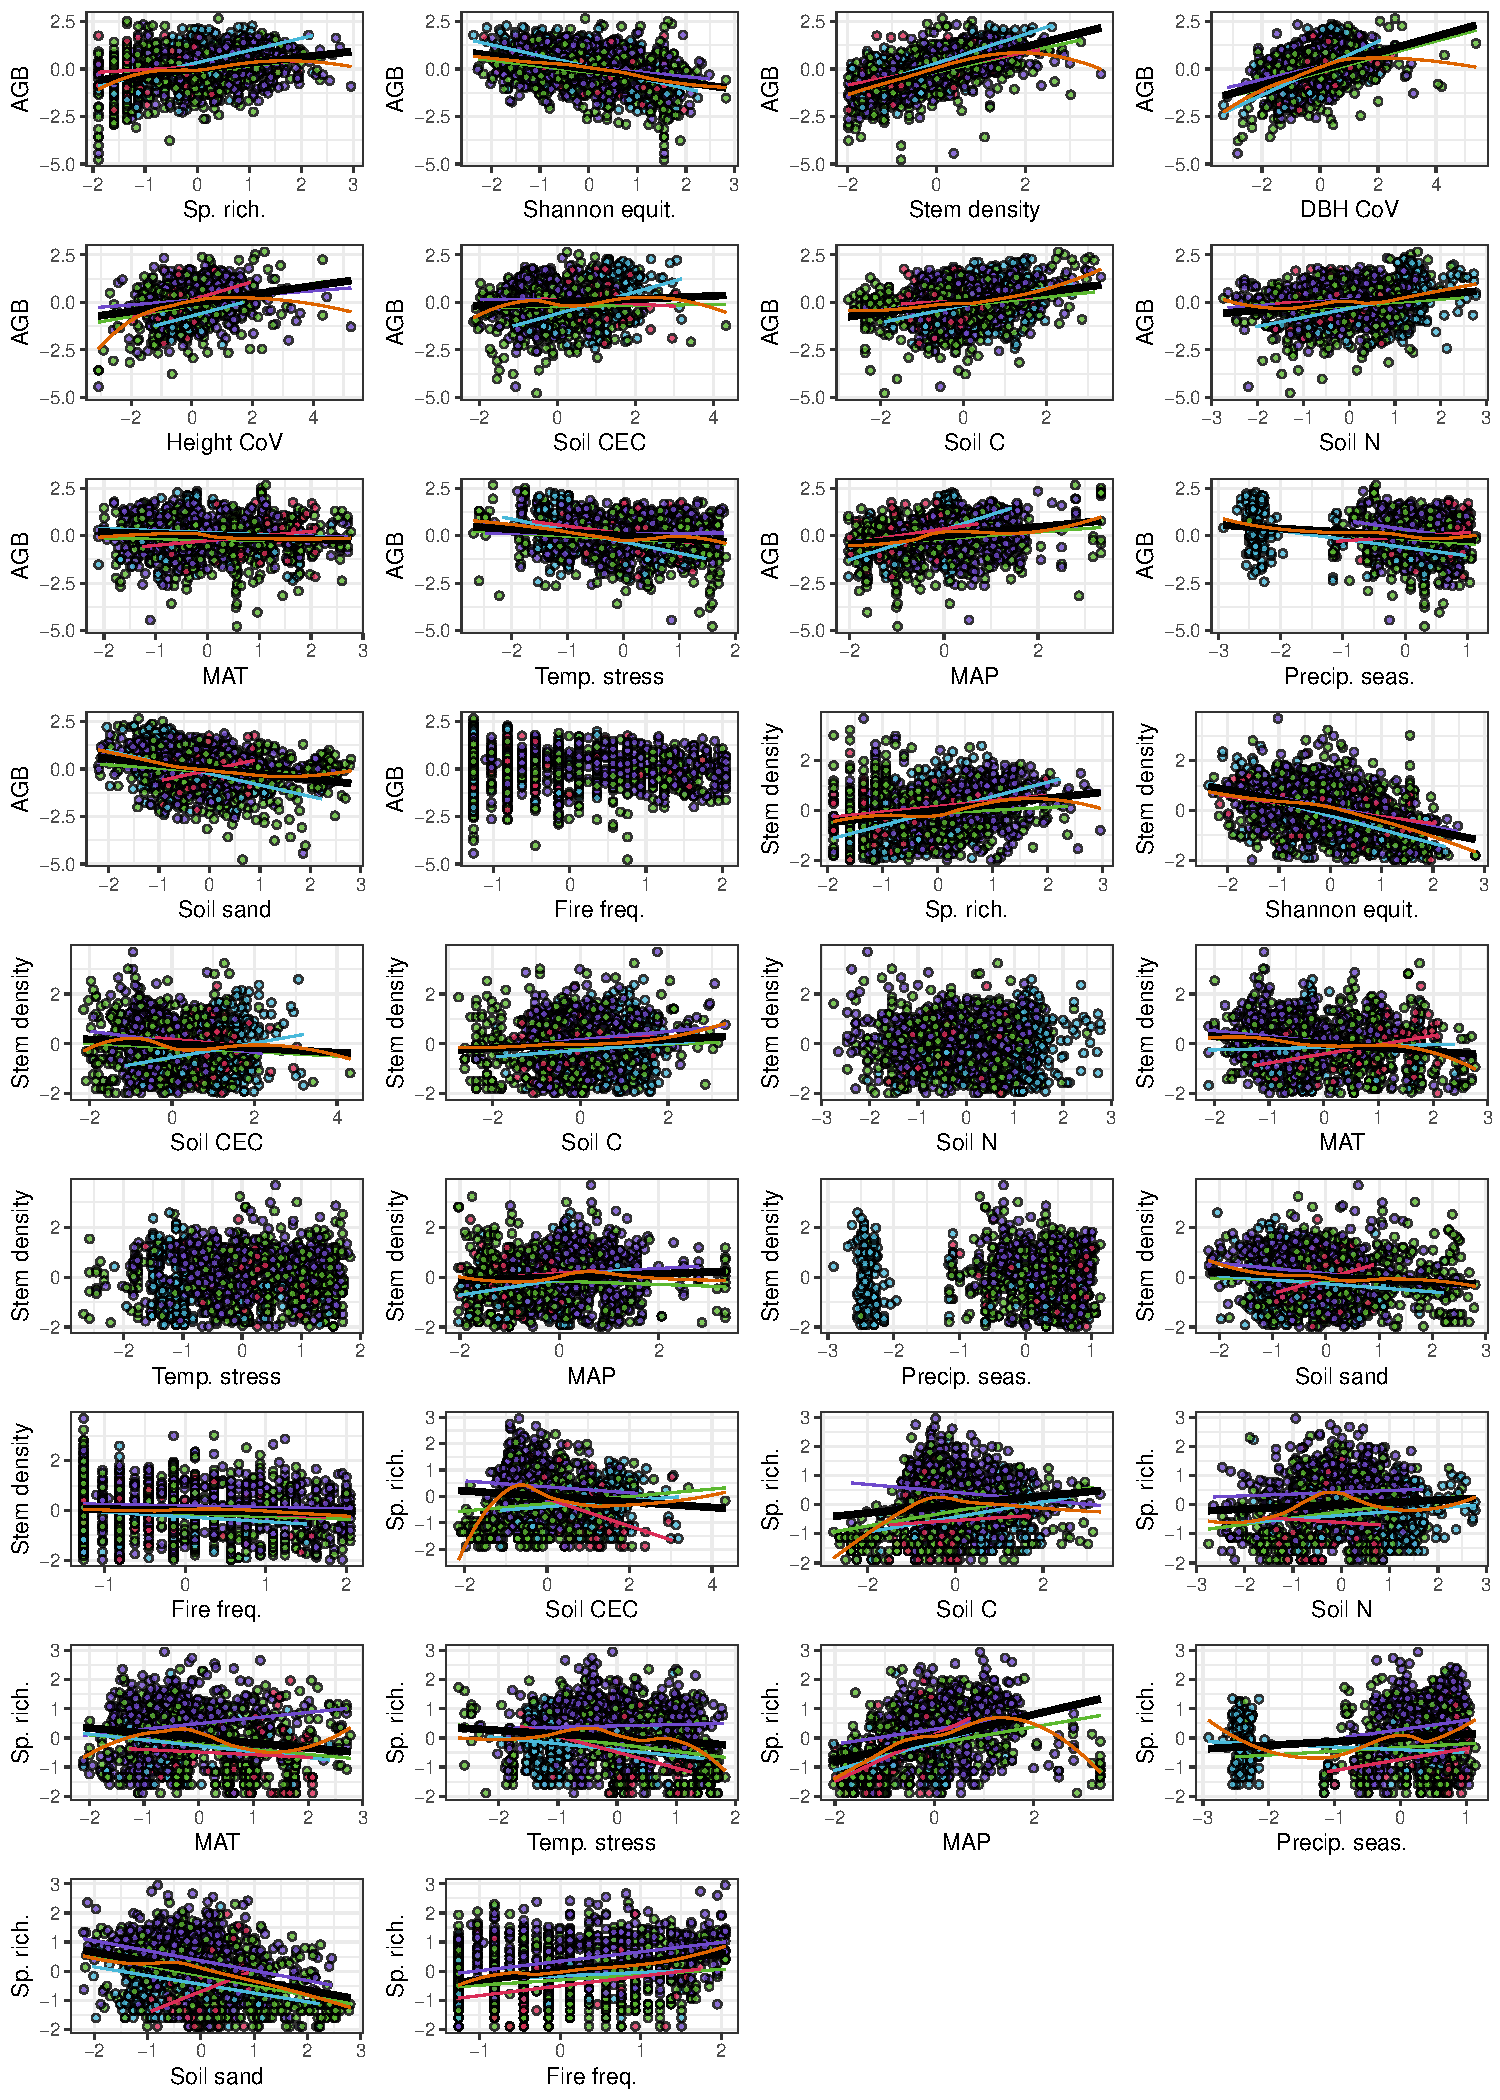
\includegraphics[width=0.9\textwidth]{bivar_lm}
	\caption{Bivariate scatter plots for each observed variable used in the SEMs, based on hypothesised paths of causality. Points are coloured according to vegetation type. A single linear regression is presented as a black line, which combines all vegetation types, separate loess trend lines are fitted for each vegetation type. An orange loess trend line is fitted for all the data. All data is standardised and variables are transformed where it was appropriate for analysis.}
	\label{bivar_lm}
\end{figure}

\section{Appendix 4 - Path coefficients for model incorporating environmental covariates} \label{appendixd}

\begin{figure}[H]
\centering
	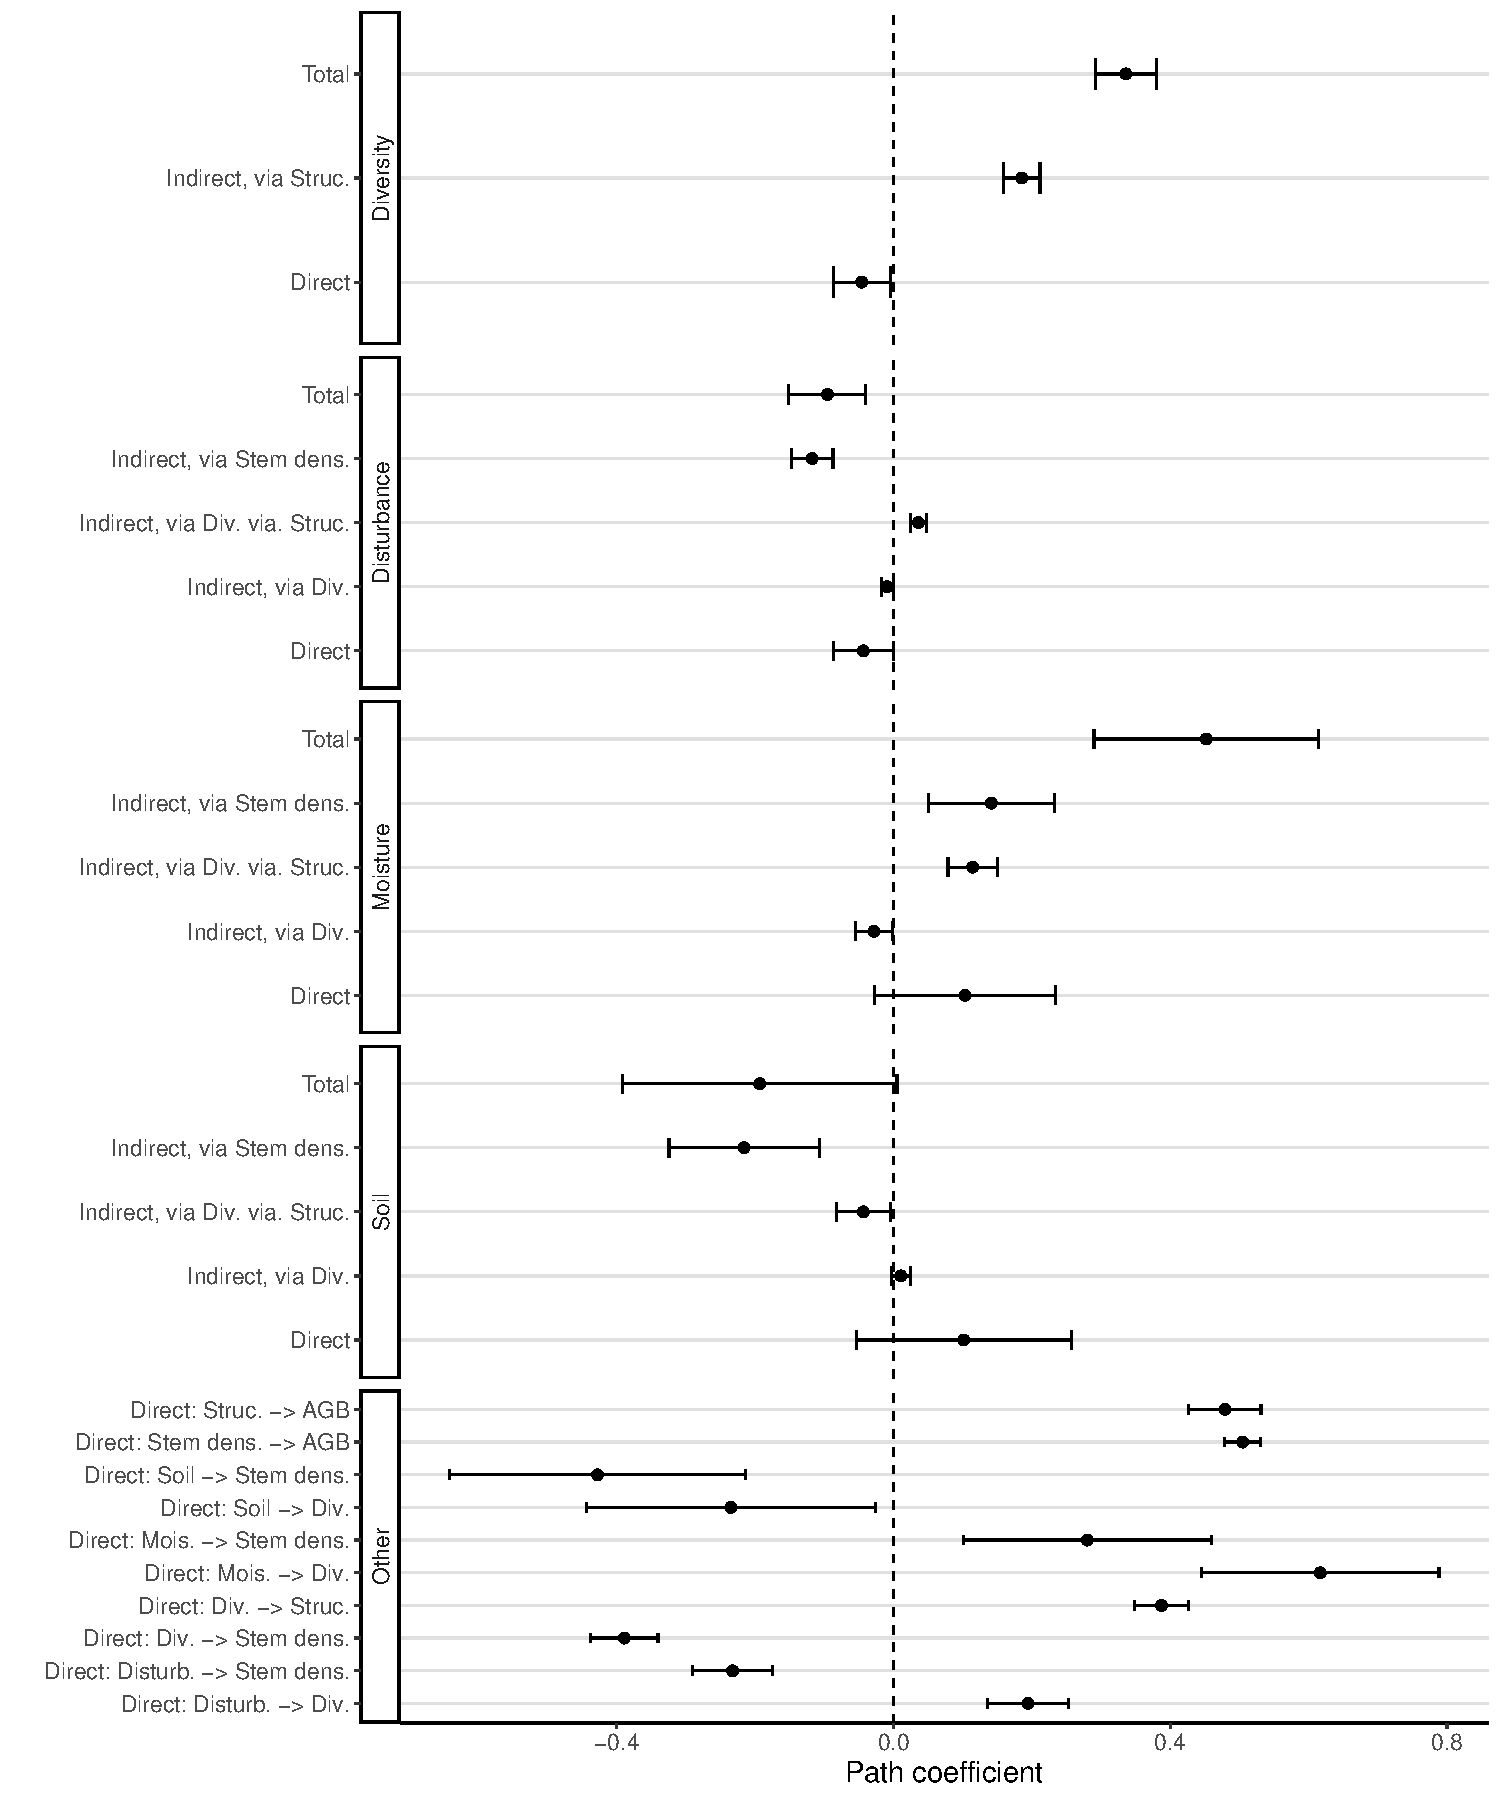
\includegraphics[width=\textwidth]{full_model_slopes}
	\caption{Unstandardised path coefficients for the full model including tree species diversity, environmental covariates and stem density. Path coefficients are $\pm1$ standard error. Path coefficients where the interval (standard error) does not overlap zero are considered to be significant effects.}
	\label{full_model_slopes}
\end{figure}

\end{document}
